\section{Fremtidig arbejde}
\begin{frame}{Scope}
Mulighed for overhaling af langsomtkørende biler
\vspace{4mm}

Tidsstyret lyssignaler
\vspace{4mm}

Kørsel uden for spidsbelastningerne
\vspace{4mm}

Biler kører efter trafikreglerne

\end{frame}

\begin{frame}{Vision}
\begin{center}
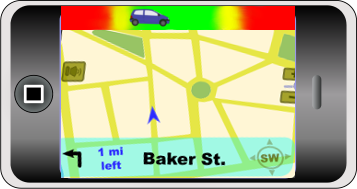
\includegraphics[width=1\textwidth]{images/product.png}
\end{center}
\end{frame}

\begin{frame}{Vision}
1. Simulering med præcise data
	\begin{itemize}
	\item Log af traffik lys
	\item Trængselsestimater (OD matrix)
	\end{itemize}

2. Smartphone applikation
	\begin{itemize}
	\item Adgang til læsning af den aktuelle signalsætning
	\end{itemize}

\end{frame}

\begin{frame}{Konklusion}
Op til 25 \% brændstofsbesparelse
\vspace{4mm}

Lav implementationsinvistering
\vspace{4mm}

Brændstofsbesparelse allerede for første køretøj
\vspace{4mm}

Individuel udbytte uafhændig af penetrationsraten
\vspace{4mm}

Minimal påvirkning af øvrig trafik
\vspace{4mm}

Mulighed for inkrementel implementering
\end{frame}
